\section{Core-periphery structure}

Previous research on Stack Exchange communities have attempted to explain how different types of users interact. In Question-Answer communities are expected popular and casual users \cite{santos2019activity, santos2019self}. Popular users generate the majority of interactions in the system, they are experts in community and take care on answering questions and engage the discussions through comments. As popular users they considered the $10 \%$ of the most active users, and showed that popular users are highly connected not only among themselves but also with casual users.

We tested this theory on all eight communities. We focused on 30 days sub-networks and showed how the number of links per node among popular users and between popular and casual users, evolve over time, figure \ref{fig:pop_cas_users}. We also compare active and closed communities of the same topic, so links per nodes in active sites are larger than in closed communities.

\begin{figure}[h!]
	\centering
	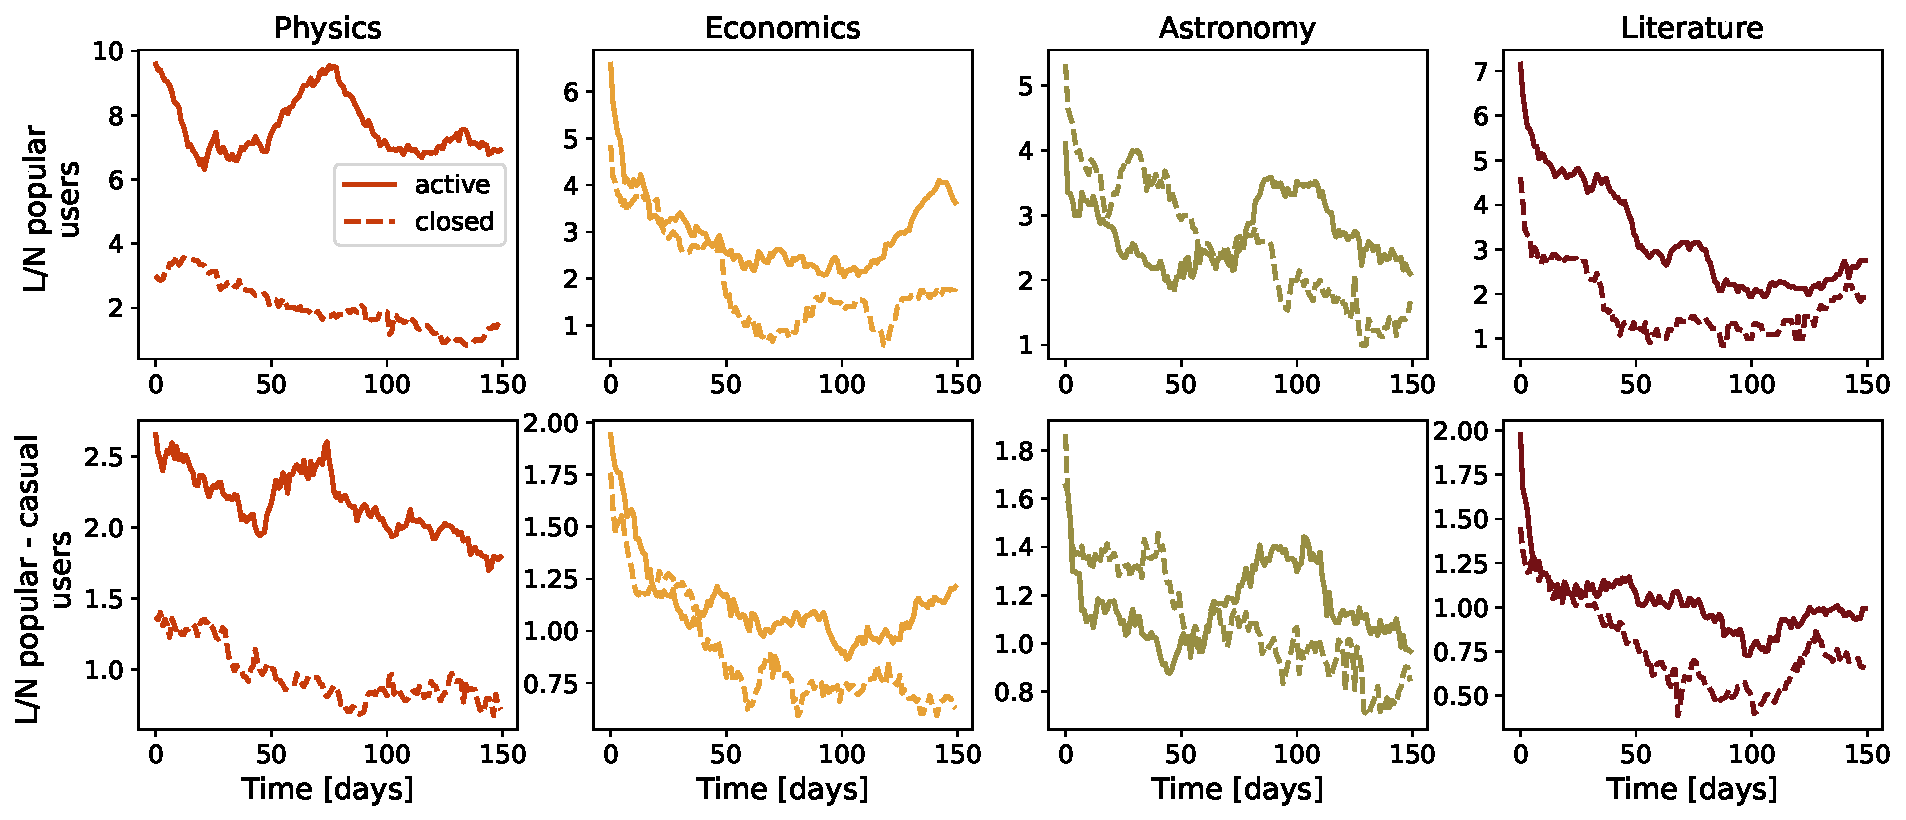
\includegraphics[width=\linewidth]{figures/stackexchange/popular_casual_users.pdf}
	\caption{Links per node among popular users (top 10\% of users) and between popular and casual users (everyone but popular users).}
	\label{fig:pop_cas_users}
\end{figure} 

Although, we find the difference between active and closed communities, the split according to $10\%$  most active users does not guaranty that all popular users will be considered. Furthermore, the smaller group of frequently active users is similar to the core users in core-periphery structure. This is why we are going to detect the core of the each 30day network. By this, separation is based on the network structure, and more consistent, as using algorithmic approach are optimized the connectivity inside the core, periphery and among them. Core-periphery structure has core that is densely connected group of nodes, while the periphery has low density \cite{fortunato2010community, gallagher2020clarified}. 

We use Stochastic Block Model (SBM) to infer the core-periphery structure of each 30 days network snapshot and analyses how core structure evolve over time.  The  SBM algorithm is adapted for inferring the core-periphery structure, \cite{gallagher2020clarified}. For each 30 days network we run the sample of 50 iterations and choose the modes parameters according to minimum description length. As stochastic models start from the random configuration, they can converge to different states. This is why we analyzed the stability of the inferred structures. More details are given in the appendix. We found that obtained structures differ, but minimum description length does not fluctuate too much. Also, different similarity measures between infered core configurations take values higher than 0.9, indicating that core structure is stable. 

\subsection{Jaccard index}

%To study the stability of the core across the time we compute Jaccard’s coefficient between core users in [t+30) networks selected at times $t_1$ and $t_2$, (figure \ref{fig:jaccard_hm}). Higher values of the Jaccard index indicate that core users tend to stay in the core. The detected cores experience a lot of change over time and the highest overlap between core users is in the network closer in the time. The average Jaccard index between core users in all sub-networks separated by time interval $|t_1 - t_2|$ with standard deviation confidence interval is presented in figure \ref{fig:jaccard_mean}. Compared to closed sites, active sites show more stability in the core. Even the number of core users obtained in the launched and closed communities are comparable \ref{fig:core_size} (a high difference is found only for physics ), the ratio between total core and periphery reputation is evidently higher in the active than in closed sites, figure \ref{fig:dr_core_per}.  

\begin{figure}[h!]
	\centering
	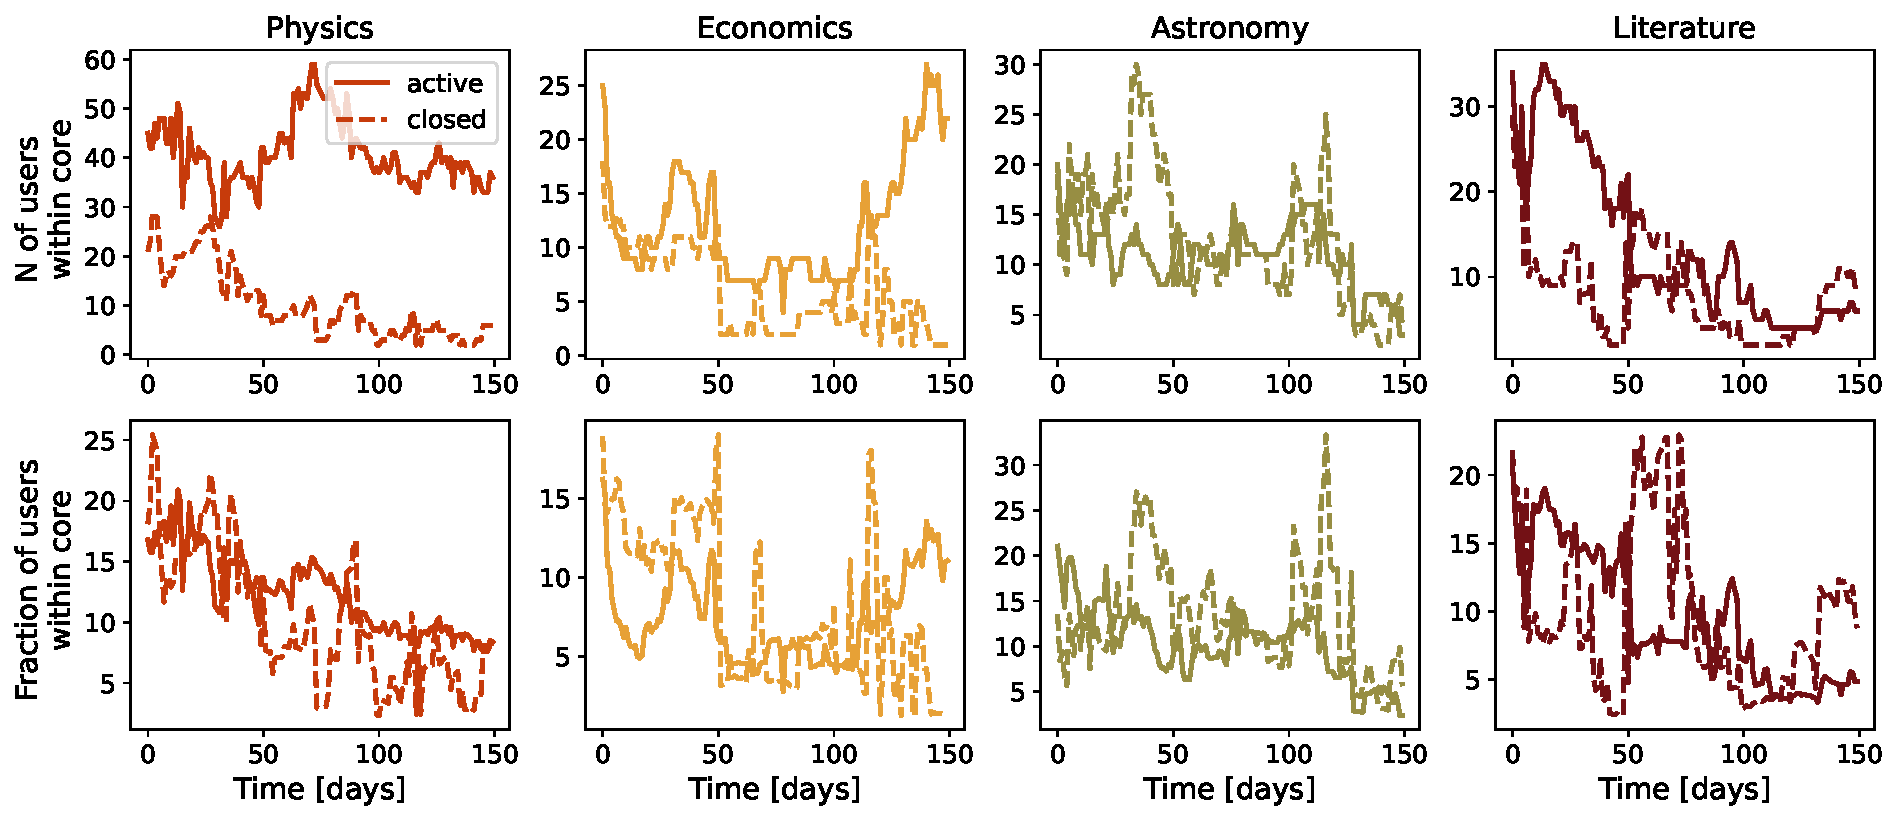
\includegraphics[width=\linewidth]{figures/stackexchange/core_users.pdf}
	\caption{Just for reference size of the core (top) and fraction of users in core (bottom). Solid lines - active sites; dashed lines - closed sites.}
	\label{fig:core_size}
\end{figure}

\begin{figure}[h!]
	\centering
	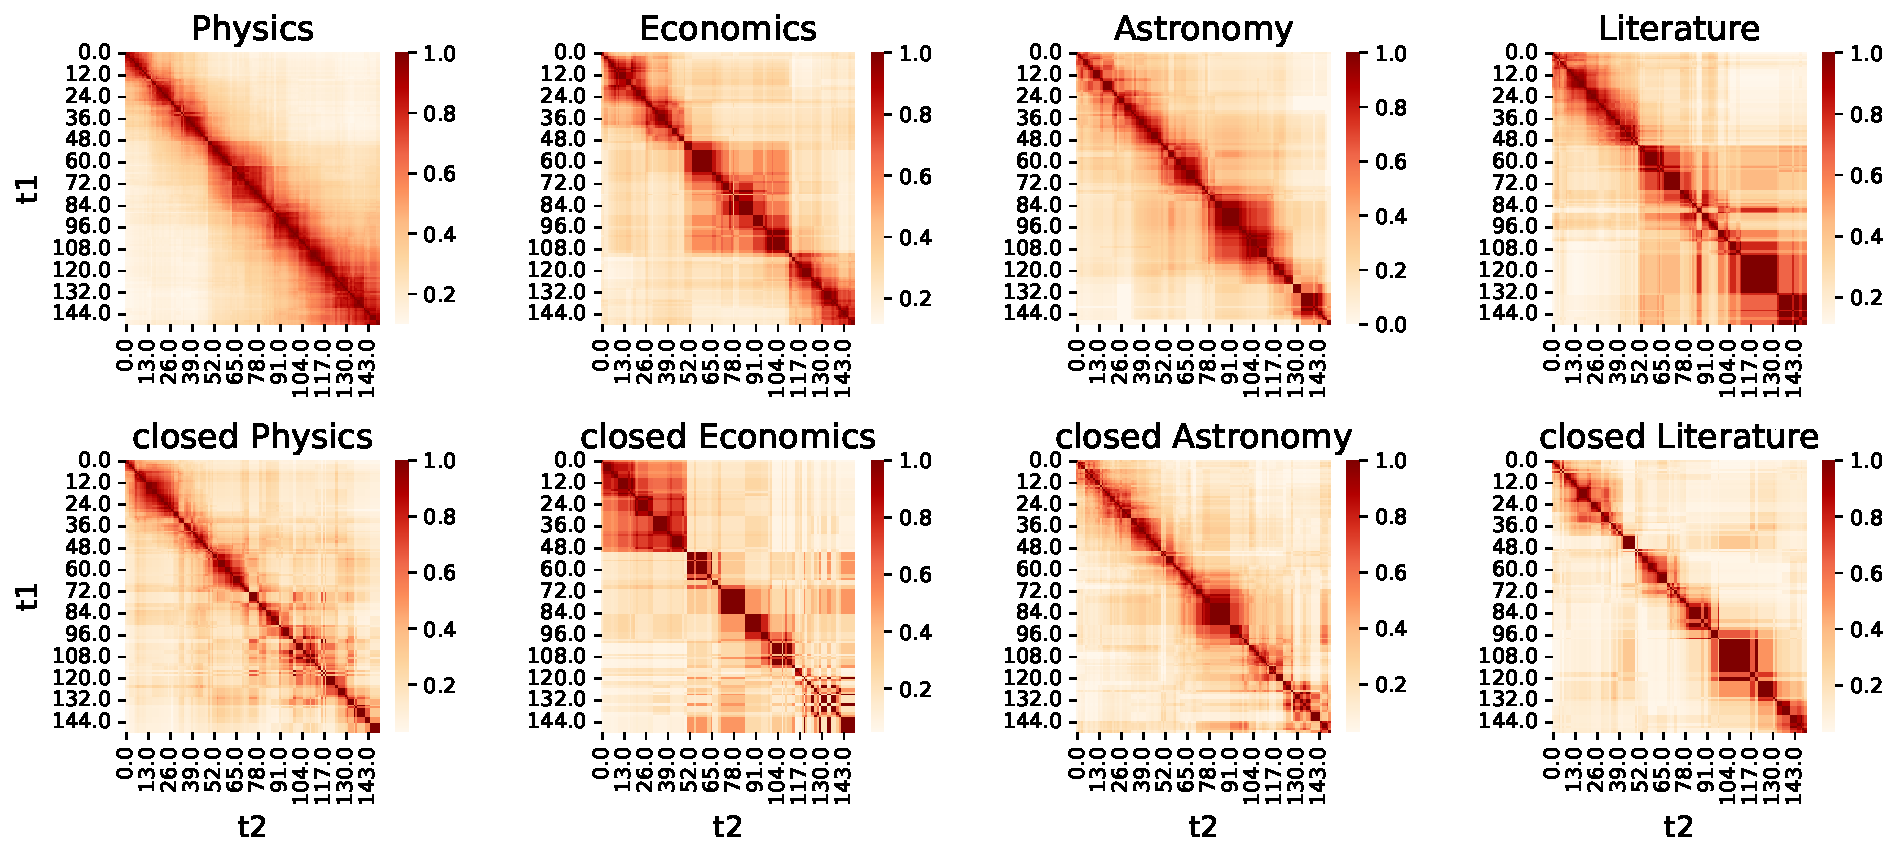
\includegraphics[width=\linewidth]{figures/stackexchange/jaccard_heatmap.pdf}
	\caption{Jaccard index between core users in  sub-networks at time points $t1$ and $t2$}
	\label{fig:jaccard_hm}
\end{figure}

\begin{figure}[h!]
	\centering
	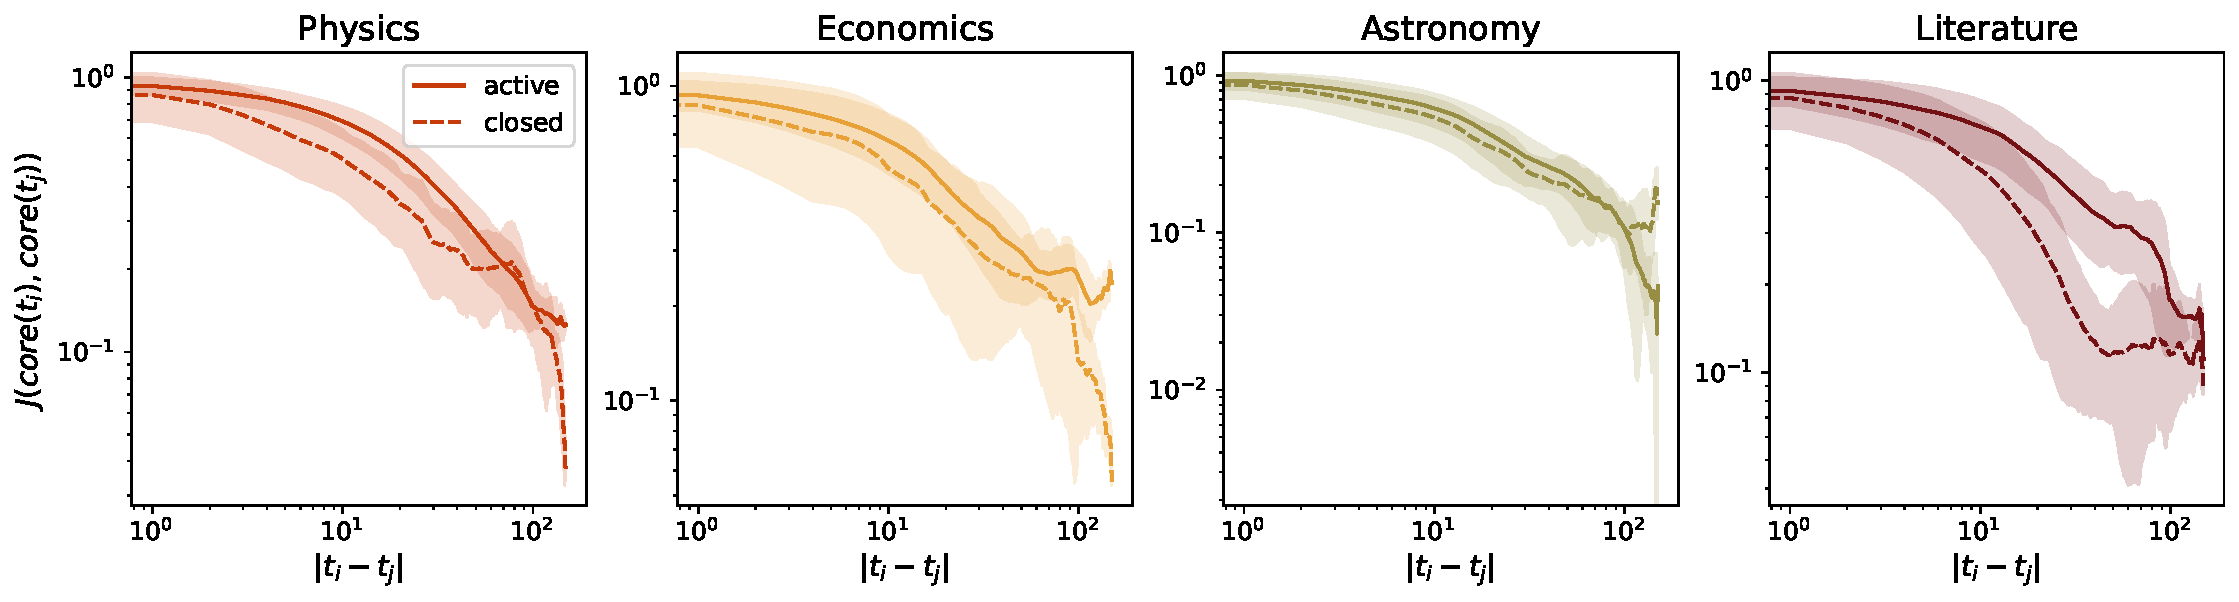
\includegraphics[width=\linewidth]{figures/stackexchange/jaccard.pdf}
	\caption{Jaccard index between core users in 30days sub-networks for all possible pairs of 30 days sub-networks separated by time interval $|t_i - t_j|$}
	\label{fig:jaccard_mean}
\end{figure}

\subsection{core-periphery density}

%Furthermore, we examine core-periphery structure of these communities and its evolution. Specifically, we are interested in the evolution of connectivity in the core. Figure \ref{fig:links_per_node} shows the number of links between nodes in the core per node $\frac{L}{N}(t)$. $\frac{2L}{N}$ is the average degree of the node in the core, and thus, $\frac{L}{N}$ is the half of the average degree. Again, Physics community has the much higher value of this quantity than Theoretical physics during the whole observed period, indicating higher connectivity between core members. Higher connectivity between core members in the active community is also characteristic for Literature, although this quantity has the same value for active and closed communities at the end of the observation period. The differences between active and closed communities are not that evident for Economics and Astronomy, see Fig. \ref{fig:links_per_node}. Active and closed Economics communities have similar connectivity in the core during the first 50 days. After this period, the connectivity in the core of the active community the twice as large as in the closed community and the difference grows at the end of observation period. The connectivity in the core of closed Astronomy community is higher that the connectivity in the core of the active community during the first 50 days. But as the time progresses, this difference changes in the favor of live community, while at the end of the observation period the difference disappears.

%The difference between active and closed communities is more prominent if we consider average number of core-periphery edges per core node. The connectivity between core and periphery is higher for the still active communities than for the closed ones, see Fig. \ref{fig:links_per_node}. This is very obvious if we compare Physics and Theoretical physics community. Moreover, Physics community has the highest connectivity compared to all other communities. When it comes to active communities that are still in the beta phase, they either have the same core-periphery connectivity as their closed counter part, or as in the case of Astronomy, their periphery is weaker connected to the core during the first 50 days of their life, see Fig. \ref{fig:links_per_node}. 

%On average, the cores of the active communities have higher number of nodes in the core than the closed communities, Fig. A11. However, the relative size of the core compared to the size of the whole network is similar when we compare closed and active communities on the same topic. This is even true for communities on physics topic. The size of the core fluctuates with time for active and closed communities. The core membership also changes with time. This core membership is changing more for the closed communities. We quantify this by calculating the Jaccard index between the cores of the subnetworks in the moment $t_{i}$ and $t_{j}$. Figure A9 in Supplementary Information shows the value of Jaccard index between any two of the 150 subnetworks. The highest value of the Jaccard index is around the diagonal and has value close to 1. This is expected, since these subnetworks are for consecutive days and the difference between them is smaller. The value of Jaccard index decreases with number of days between two subnetworks $|t_{i}-t_{j}|$ faster in closed communities Fig. A10. This difference is the most prominent for the literature communities, while this difference is practically non-existent for Astronomy. The relatively high overlap between cores of even more distant subnetworks for active communities, further confirms that the core is more stable in these communities that in their closed counterparts. 

\begin{figure}[h]
	\centering
	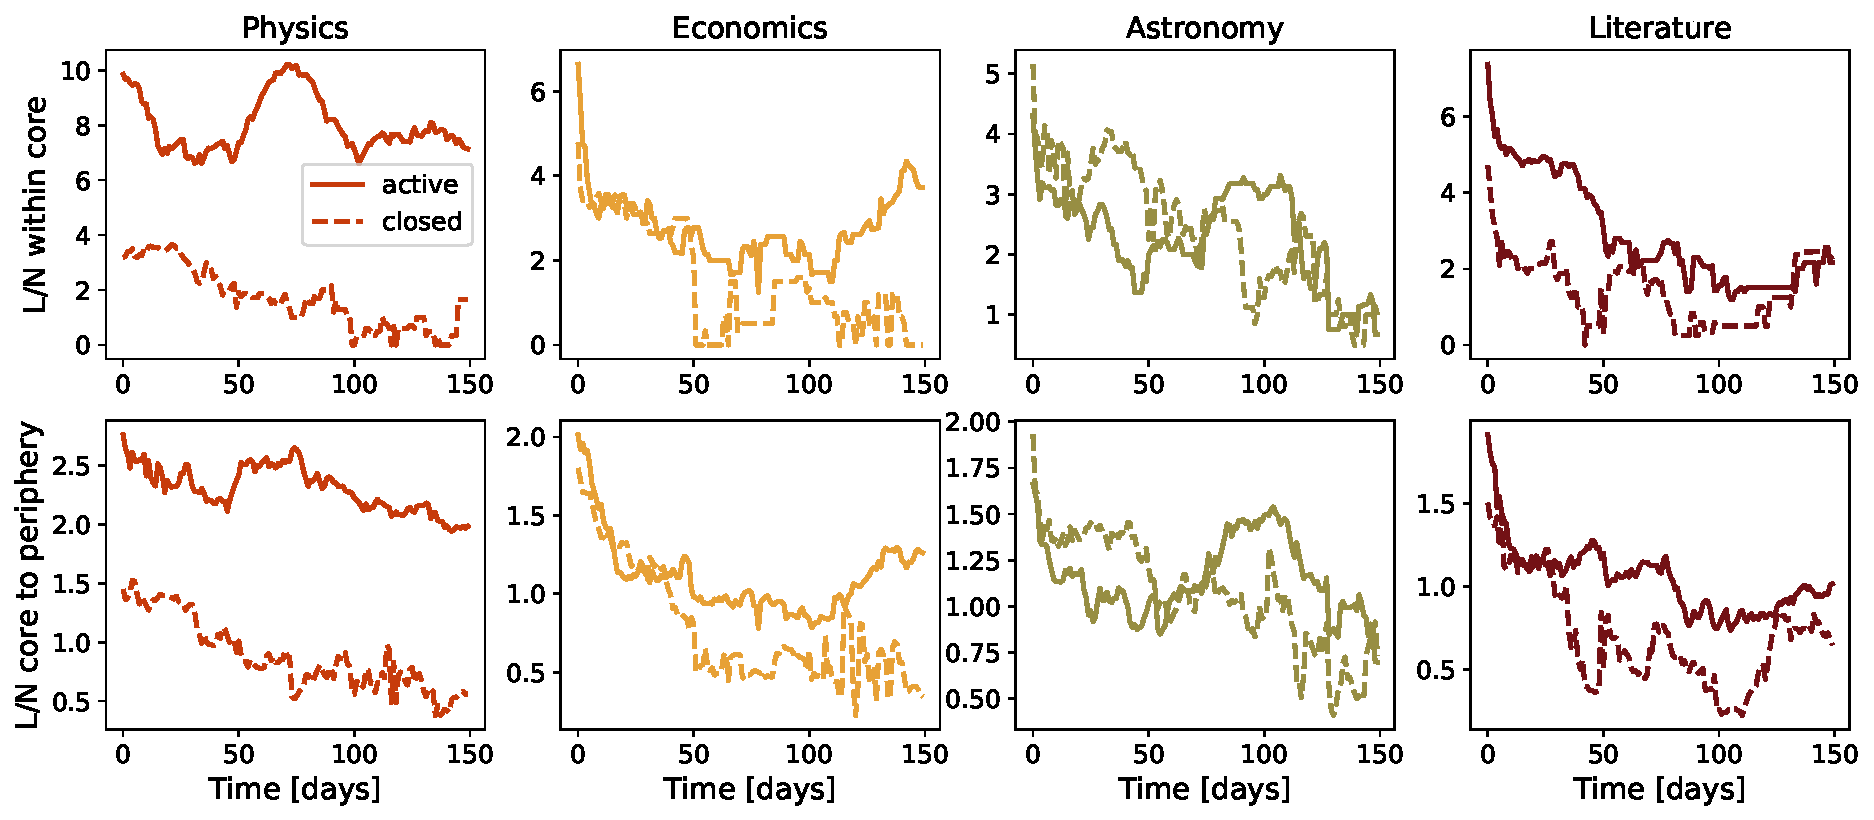
\includegraphics[width=\linewidth]{figures/stackexchange/core_connectivity.pdf}
	\caption{Links per node in core and links per node between core and periphery.}
	\label{fig:links_per_node}
\end{figure}

